% Options for packages loaded elsewhere
\PassOptionsToPackage{unicode}{hyperref}
\PassOptionsToPackage{hyphens}{url}
%
\documentclass[
  english,
  man]{apa6}
\usepackage{lmodern}
\usepackage{amssymb,amsmath}
\usepackage{ifxetex,ifluatex}
\ifnum 0\ifxetex 1\fi\ifluatex 1\fi=0 % if pdftex
  \usepackage[T1]{fontenc}
  \usepackage[utf8]{inputenc}
  \usepackage{textcomp} % provide euro and other symbols
\else % if luatex or xetex
  \usepackage{unicode-math}
  \defaultfontfeatures{Scale=MatchLowercase}
  \defaultfontfeatures[\rmfamily]{Ligatures=TeX,Scale=1}
\fi
% Use upquote if available, for straight quotes in verbatim environments
\IfFileExists{upquote.sty}{\usepackage{upquote}}{}
\IfFileExists{microtype.sty}{% use microtype if available
  \usepackage[]{microtype}
  \UseMicrotypeSet[protrusion]{basicmath} % disable protrusion for tt fonts
}{}
\makeatletter
\@ifundefined{KOMAClassName}{% if non-KOMA class
  \IfFileExists{parskip.sty}{%
    \usepackage{parskip}
  }{% else
    \setlength{\parindent}{0pt}
    \setlength{\parskip}{6pt plus 2pt minus 1pt}}
}{% if KOMA class
  \KOMAoptions{parskip=half}}
\makeatother
\usepackage{xcolor}
\IfFileExists{xurl.sty}{\usepackage{xurl}}{} % add URL line breaks if available
\IfFileExists{bookmark.sty}{\usepackage{bookmark}}{\usepackage{hyperref}}
\hypersetup{
  pdftitle={Lab 8 Group Committing to github},
  pdfauthor={Janette Avelar1, David Fainstein1, Joe Swinehart1, \& Makayla Whitney1},
  pdflang={en-EN},
  pdfkeywords={teacher, experience, lunch, math, scores},
  hidelinks,
  pdfcreator={LaTeX via pandoc}}
\urlstyle{same} % disable monospaced font for URLs
\usepackage{graphicx,grffile}
\makeatletter
\def\maxwidth{\ifdim\Gin@nat@width>\linewidth\linewidth\else\Gin@nat@width\fi}
\def\maxheight{\ifdim\Gin@nat@height>\textheight\textheight\else\Gin@nat@height\fi}
\makeatother
% Scale images if necessary, so that they will not overflow the page
% margins by default, and it is still possible to overwrite the defaults
% using explicit options in \includegraphics[width, height, ...]{}
\setkeys{Gin}{width=\maxwidth,height=\maxheight,keepaspectratio}
% Set default figure placement to htbp
\makeatletter
\def\fps@figure{htbp}
\makeatother
\setlength{\emergencystretch}{3em} % prevent overfull lines
\providecommand{\tightlist}{%
  \setlength{\itemsep}{0pt}\setlength{\parskip}{0pt}}
\setcounter{secnumdepth}{-\maxdimen} % remove section numbering
% Make \paragraph and \subparagraph free-standing
\ifx\paragraph\undefined\else
  \let\oldparagraph\paragraph
  \renewcommand{\paragraph}[1]{\oldparagraph{#1}\mbox{}}
\fi
\ifx\subparagraph\undefined\else
  \let\oldsubparagraph\subparagraph
  \renewcommand{\subparagraph}[1]{\oldsubparagraph{#1}\mbox{}}
\fi
% Manuscript styling
\usepackage{upgreek}
\captionsetup{font=singlespacing,justification=justified}

% Table formatting
\usepackage{longtable}
\usepackage{lscape}
% \usepackage[counterclockwise]{rotating}   % Landscape page setup for large tables
\usepackage{multirow}		% Table styling
\usepackage{tabularx}		% Control Column width
\usepackage[flushleft]{threeparttable}	% Allows for three part tables with a specified notes section
\usepackage{threeparttablex}            % Lets threeparttable work with longtable

% Create new environments so endfloat can handle them
% \newenvironment{ltable}
%   {\begin{landscape}\begin{center}\begin{threeparttable}}
%   {\end{threeparttable}\end{center}\end{landscape}}
\newenvironment{lltable}{\begin{landscape}\begin{center}\begin{ThreePartTable}}{\end{ThreePartTable}\end{center}\end{landscape}}

% Enables adjusting longtable caption width to table width
% Solution found at http://golatex.de/longtable-mit-caption-so-breit-wie-die-tabelle-t15767.html
\makeatletter
\newcommand\LastLTentrywidth{1em}
\newlength\longtablewidth
\setlength{\longtablewidth}{1in}
\newcommand{\getlongtablewidth}{\begingroup \ifcsname LT@\roman{LT@tables}\endcsname \global\longtablewidth=0pt \renewcommand{\LT@entry}[2]{\global\advance\longtablewidth by ##2\relax\gdef\LastLTentrywidth{##2}}\@nameuse{LT@\roman{LT@tables}} \fi \endgroup}

% \setlength{\parindent}{0.5in}
% \setlength{\parskip}{0pt plus 0pt minus 0pt}

% \usepackage{etoolbox}
\makeatletter
\patchcmd{\HyOrg@maketitle}
  {\section{\normalfont\normalsize\abstractname}}
  {\section*{\normalfont\normalsize\abstractname}}
  {}{\typeout{Failed to patch abstract.}}
\patchcmd{\HyOrg@maketitle}
  {\section{\protect\normalfont{\@title}}}
  {\section*{\protect\normalfont{\@title}}}
  {}{\typeout{Failed to patch title.}}
\makeatother
\shorttitle{pay no attention to the tibble behind the curtain}
\keywords{teacher, experience, lunch, math, scores}
\DeclareDelayedFloatFlavor{ThreePartTable}{table}
\DeclareDelayedFloatFlavor{lltable}{table}
\DeclareDelayedFloatFlavor*{longtable}{table}
\makeatletter
\renewcommand{\efloat@iwrite}[1]{\immediate\expandafter\protected@write\csname efloat@post#1\endcsname{}}
\makeatother
\usepackage{csquotes}
\ifxetex
  % Load polyglossia as late as possible: uses bidi with RTL langages (e.g. Hebrew, Arabic)
  \usepackage{polyglossia}
  \setmainlanguage[]{english}
\else
  \usepackage[shorthands=off,main=english]{babel}
\fi

\title{Lab 8 Group Committing to github}
\author{Janette Avelar\textsuperscript{1}, David Fainstein\textsuperscript{1}, Joe Swinehart\textsuperscript{1}, \& Makayla Whitney\textsuperscript{1}}
\date{}


\authornote{

Janette Avelar, University of Oregon College of Education,
David Fainstein, University of Oregon College of Education,
Joe Swinehart, Behavioral Research \& Teaching,
Makayla Whitney, University of Oregon College of Education

Project completed using RStudio, GitKraken, GitHub, and papaja

Contact: \href{mailto:javelar7@uoregon.edu}{\nolinkurl{javelar7@uoregon.edu}}

The authors made the following contributions. Janette Avelar: Writing - Review \& Committing; David Fainstein: Writing - Review \& Committing; Joe Swinehart: Writing - Review \& Committing; Makayla Whitney: Writing - Review \& Committing.

Correspondence concerning this article should be addressed to Janette Avelar, Oregon, USA. E-mail: \href{mailto:javelar7@uoregon.edu}{\nolinkurl{javelar7@uoregon.edu}}

}

\affiliation{\vspace{0.5cm}\textsuperscript{1} University of Oregon}

\abstract{
This project aims to explore the relationship between teacher experience and student math scores, with an additional look at how free/reduced price lunch status correpsonds to that relationship.
}



\begin{document}
\maketitle

\begin{verbatim}
## # A tibble: 4 x 6
## # Groups:   sex [2]
##   sex   frl   math_mean math_sd read_mean read_ss
##   <chr> <chr>     <dbl>   <dbl>     <dbl>   <dbl>
## 1 boy   no         493.    46.3      441.    32.3
## 2 boy   yes        470.    46.1      425.    26.6
## 3 girl  no         501.    46.0      449.    34.5
## 4 girl  yes        478.    46.3      431.    27.4
\end{verbatim}

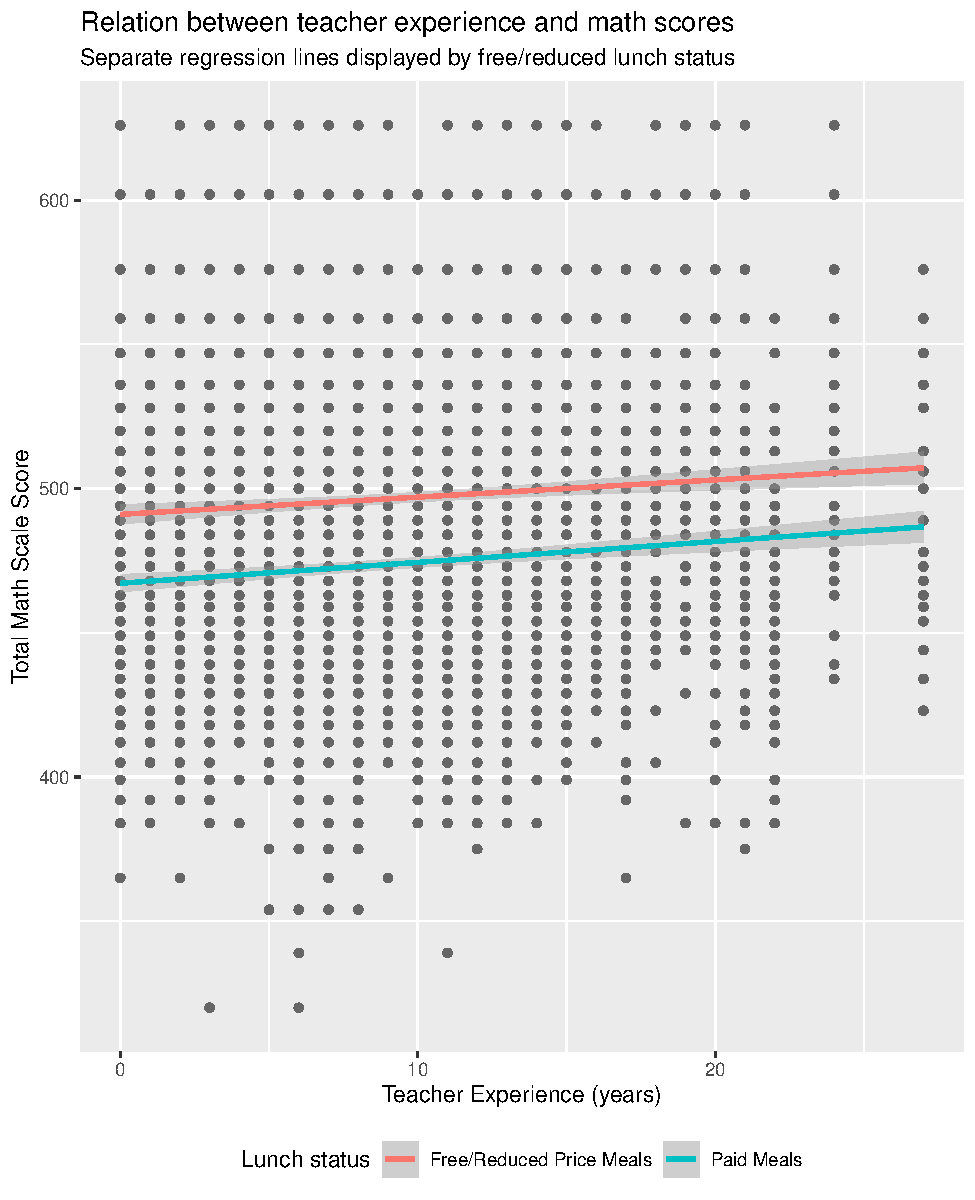
\includegraphics{lab_8_files/figure-latex/graph-1.pdf}

\hypertarget{summary-statistics-table}{%
\section{Summary Statistics Table}\label{summary-statistics-table}}

\hypertarget{methods}{%
\section{Methods}\label{methods}}

We report how we determined our sample size, all data exclusions (if any), all manipulations, and all measures in the study.

\hypertarget{participants}{%
\subsection{Participants}\label{participants}}

There were some people involved.

\hypertarget{material}{%
\subsection{Material}\label{material}}

Here's some words.

\hypertarget{procedure}{%
\subsection{Procedure}\label{procedure}}

We did things and we did them well.

\hypertarget{data-analysis}{%
\subsection{Data analysis}\label{data-analysis}}

We used R (Version 4.0.2; R Core Team, 2020b) and the R-packages \emph{\}dplyr} {[}@\}R-dplyr{]}, \emph{forcats} (Version 0.5.0; Wickham, 2020a), \emph{foreign} (Version 0.8.80; R Core Team, 2020a), \emph{ggplot2} (Version 3.3.2; Wickham, 2016), \emph{here} (Version 0.1; Müller, 2017), \emph{openxlsx} (Version 4.2.2; Schauberger \& Walker, 2020), \emph{packrat} (Ushey, McPherson, Cheng, Atkins, \& Allaire, 2018), \emph{papaja} (Version 0.1.0.9997; Aust \& Barth, 2020), \emph{purrr} (Version 0.3.4; Henry \& Wickham, 2020), \emph{readr} (Version 1.4.0; Wickham \& Hester, 2020), \emph{rio} (Version 0.5.16; Chan, Chan, Leeper, \& Becker, 2018), \emph{stringr} (Version 1.4.0; Wickham, 2019), \emph{tibble} (Version 3.0.4; Müller \& Wickham, 2020), \emph{tidyr} (Version 1.1.2; Wickham, 2020b), and \emph{tidyverse} (Version 1.3.0; Wickham et al., 2019) for all our analyses.

There was some data gathered and it was neat.

\hypertarget{results}{%
\section{Results}\label{results}}

\hypertarget{discussion}{%
\section{Discussion}\label{discussion}}

This fits into O'neil (2016) discussion about math stuff, we think. We didn't actually read it, but liked the name \emph{Weapons of Math Destruction}.

Another article we didn't read investigates children's understanding of math and science, by Lehrer and Schauble (2002). It seems cool.

\newpage

\hypertarget{references}{%
\section{References}\label{references}}

\begingroup
\setlength{\parindent}{-0.5in}
\setlength{\leftskip}{0.5in}

\hypertarget{refs}{}
\leavevmode\hypertarget{ref-R-papaja}{}%
Aust, F., \& Barth, M. (2020). \emph{papaja: Create APA manuscripts with R Markdown}. Retrieved from \url{https://github.com/crsh/papaja}

\leavevmode\hypertarget{ref-R-rio}{}%
Chan, C.-h., Chan, G. C., Leeper, T. J., \& Becker, J. (2018). \emph{Rio: A swiss-army knife for data file i/o}.

\leavevmode\hypertarget{ref-R-purrr}{}%
Henry, L., \& Wickham, H. (2020). \emph{Purrr: Functional programming tools}. Retrieved from \url{https://CRAN.R-project.org/package=purrr}

\leavevmode\hypertarget{ref-lehrer_children}{}%
Lehrer, R., \& Schauble, L. (2002). \emph{Investigating real data in the classroom: Expanding children's understanding of math and science. Ways of knowing in science and mathematics series.} ERIC.

\leavevmode\hypertarget{ref-R-here}{}%
Müller, K. (2017). \emph{Here: A simpler way to find your files}. Retrieved from \url{https://CRAN.R-project.org/package=here}

\leavevmode\hypertarget{ref-R-tibble}{}%
Müller, K., \& Wickham, H. (2020). \emph{Tibble: Simple data frames}. Retrieved from \url{https://CRAN.R-project.org/package=tibble}

\leavevmode\hypertarget{ref-oneil_weapons}{}%
O'neil, C. (2016). \emph{Weapons of math destruction: How big data increases inequality and threatens democracy}. Broadway Books.

\leavevmode\hypertarget{ref-R-foreign}{}%
R Core Team. (2020a). \emph{Foreign: Read data stored by 'minitab', 's', 'sas', 'spss', 'stata', 'systat', 'weka', 'dBase', ...} Retrieved from \url{https://CRAN.R-project.org/package=foreign}

\leavevmode\hypertarget{ref-R-base}{}%
R Core Team. (2020b). \emph{R: A language and environment for statistical computing}. Vienna, Austria: R Foundation for Statistical Computing. Retrieved from \url{https://www.R-project.org/}

\leavevmode\hypertarget{ref-R-openxlsx}{}%
Schauberger, P., \& Walker, A. (2020). \emph{Openxlsx: Read, write and edit xlsx files}. Retrieved from \url{https://CRAN.R-project.org/package=openxlsx}

\leavevmode\hypertarget{ref-R-packrat}{}%
Ushey, K., McPherson, J., Cheng, J., Atkins, A., \& Allaire, J. (2018). \emph{Packrat: A dependency management system for projects and their r package dependencies}. Retrieved from \url{https://CRAN.R-project.org/package=packrat}

\leavevmode\hypertarget{ref-R-ggplot2}{}%
Wickham, H. (2016). \emph{Ggplot2: Elegant graphics for data analysis}. Springer-Verlag New York. Retrieved from \url{https://ggplot2.tidyverse.org}

\leavevmode\hypertarget{ref-R-stringr}{}%
Wickham, H. (2019). \emph{Stringr: Simple, consistent wrappers for common string operations}. Retrieved from \url{https://CRAN.R-project.org/package=stringr}

\leavevmode\hypertarget{ref-R-forcats}{}%
Wickham, H. (2020a). \emph{Forcats: Tools for working with categorical variables (factors)}. Retrieved from \url{https://CRAN.R-project.org/package=forcats}

\leavevmode\hypertarget{ref-R-tidyr}{}%
Wickham, H. (2020b). \emph{Tidyr: Tidy messy data}. Retrieved from \url{https://CRAN.R-project.org/package=tidyr}

\leavevmode\hypertarget{ref-R-tidyverse}{}%
Wickham, H., Averick, M., Bryan, J., Chang, W., McGowan, L. D., François, R., \ldots{} Yutani, H. (2019). Welcome to the tidyverse. \emph{Journal of Open Source Software}, \emph{4}(43), 1686. \url{https://doi.org/10.21105/joss.01686}

\leavevmode\hypertarget{ref-R-readr}{}%
Wickham, H., \& Hester, J. (2020). \emph{Readr: Read rectangular text data}. Retrieved from \url{https://CRAN.R-project.org/package=readr}

\endgroup


\end{document}
